\documentclass[11pt]{article}
\usepackage[notes]{la}
\lamodule{5}{4}{Eigenvectors and Linear Transformations}
\laxdoc{1.8}
\laxdoc{1.9}
\laxdoc{2.2}
\laxdoc{2.3}
\laxdoc{4.2}
\laxdoc{4.3}
\laxdoc{4.4}

\begin{document}

\section{Eigenvectors and Linear Transformations}

\begin{guide}
A vector has no coordinates of its own. It acquires coordinates only when we choose a basis, and a different basis gives different numbers for the same vector. A linear transformation is in the same position: its matrix depends on the bases we use to describe the input and the output. This section answers two questions that come from Section~4.4. How do the two coordinate vectors of one vector, in two different bases, determine each other? And how do we write a linear transformation as a matrix when the bases are not the standard ones? The answers are two matrix constructions, both built column by column from coordinate vectors. At the end we meet the best possible case: a basis in which the matrix of a transformation is diagonal, so that the transformation just scales each basis vector.
\end{guide}

\textbf{By the end of this section you should be able to:}
\begin{itemize}
  \item find the change-of-basis matrix between two bases of $\R^n$, $\mathbb{P}_n$ or another space with coordinates, and use it to convert coordinate vectors in both directions;
  \item explain why the change-of-basis matrix is invertible and why its inverse is the matrix that changes coordinates the other way;
  \item find the matrix of a linear transformation relative to a basis of the domain and a basis of the codomain, and use it to compute images in coordinates;
  \item find the matrix of $\bv{x}\mapsto A\bv{x}$ relative to a basis $\mathcal{B}$ of $\R^n$, and explain the formula $P_{\mathcal{B}}^{-1}AP_{\mathcal{B}}$;
  \item relate the matrices of one transformation in two different bases;
  \item recognize when a matrix of a transformation is diagonal, say what the transformation does to each basis vector, and build or find such a basis.
\end{itemize}

% ---------------------------------------------------------------------
\subsection*{One vector, two coordinate vectors}

Section~4.4 gave us the coordinate vector $[\bv{x}]_{\mathcal{B}}$ of a vector $\bv{x}$ relative to a basis $\mathcal{B}$ (Definition~\ref{4.4-def:coords}), and the fact that the coordinate mapping $\bv{x}\mapsto[\bv{x}]_{\mathcal{B}}$ is linear (Theorem~\ref{4.4-thm:coordmap}). Linear maps of coordinate vectors are matrix maps, so we should expect that going from one set of coordinates to another is a matrix multiplication. Here is a first look at one case.

\begin{exmp}{The same vector in two bases}{twocoords}
Let $\mathcal{B}=\{\bv{b}_1,\bv{b}_2\}$ with $\bv{b}_1=(2,1)$, $\bv{b}_2=(1,1)$, let $\mathcal{C}=\{\bv{c}_1,\bv{c}_2\}$ with $\bv{c}_1=(1,3)$, $\bv{c}_2=(0,1)$, and let $\bv{x}=(4,3)$. Solving $2c_1+c_2=4$, $c_1+c_2=3$ gives $[\bv{x}]_{\mathcal{B}}=(1,2)$: indeed $1\cdot(2,1)+2\cdot(1,1)=(4,3)$. Solving $c_1(1,3)+c_2(0,1)=(4,3)$ gives $c_1=4$ and $c_2=3-12=-9$, so $[\bv{x}]_{\mathcal{C}}=(4,-9)$. The two coordinate vectors are different, but each one determines the other. To find the rule, write the vectors of $\mathcal{B}$ in $\mathcal{C}$-coordinates: $\bv{b}_1=(2,1)=2\bv{c}_1-5\bv{c}_2$, because $2(1,3)-5(0,1)=(2,1)$; and $\bv{b}_2=(1,1)=1\cdot\bv{c}_1-2\bv{c}_2$. So $[\bv{b}_1]_{\mathcal{C}}=(2,-5)$ and $[\bv{b}_2]_{\mathcal{C}}=(1,-2)$. Now $\bv{x}=1\cdot\bv{b}_1+2\bv{b}_2$, and the coordinate mapping is linear, so
\[
[\bv{x}]_{\mathcal{C}}=1\cdot[\bv{b}_1]_{\mathcal{C}}+2\,[\bv{b}_2]_{\mathcal{C}}=\begin{bmatrix}2&1\\-5&-2\end{bmatrix}\begin{bmatrix}1\\2\end{bmatrix}=\begin{bmatrix}4\\-9\end{bmatrix}.
\]
The matrix $\begin{bmatrix}2&1\\-5&-2\end{bmatrix}$, whose columns are the $\mathcal{C}$-coordinates of the vectors of $\mathcal{B}$, turned $[\bv{x}]_{\mathcal{B}}$ into $[\bv{x}]_{\mathcal{C}}$. Nothing in it depended on the choice $\bv{x}=(4,3)$.
\end{exmp}

\begin{defn}{Change-of-basis matrix}{pcb}
Let $\mathcal{B}=\{\bv{b}_1,\dots,\bv{b}_n\}$ and $\mathcal{C}=\{\bv{c}_1,\dots,\bv{c}_n\}$ be two bases of the same vector space $V$. The \emph{change-of-basis matrix from $\mathcal{B}$ to $\mathcal{C}$} is the $n\times n$ matrix
\[
P_{\mathcal{C}\leftarrow\mathcal{B}}=\begin{bmatrix}[\bv{b}_1]_{\mathcal{C}}&[\bv{b}_2]_{\mathcal{C}}&\cdots&[\bv{b}_n]_{\mathcal{C}}\end{bmatrix},
\]
whose $j$th column is the $\mathcal{C}$-coordinate vector of the $j$th vector of $\mathcal{B}$.
\end{defn}

The notation is meant to be read from right to left, like a composition of functions: $P_{\mathcal{C}\leftarrow\mathcal{B}}$ takes $\mathcal{B}$-coordinates as input and gives $\mathcal{C}$-coordinates as output. The matrix of Example~\ref{ex:twocoords} is $P_{\mathcal{C}\leftarrow\mathcal{B}}$.

\begin{thm}{Changing coordinates}{change}
Let $\mathcal{B}$ and $\mathcal{C}$ be bases of the vector space $V$, each with $n$ vectors. Then
\begin{enumerate}[label=(\alph*),itemsep=1pt]
  \item $[\bv{x}]_{\mathcal{C}}=P_{\mathcal{C}\leftarrow\mathcal{B}}\,[\bv{x}]_{\mathcal{B}}$ for every $\bv{x}$ in $V$;
  \item $P_{\mathcal{C}\leftarrow\mathcal{B}}$ is invertible, and its inverse is $P_{\mathcal{B}\leftarrow\mathcal{C}}$.
\end{enumerate}
\end{thm}

\begin{proof}
(a)~Write $\bv{x}=c_1\bv{b}_1+\cdots+c_n\bv{b}_n$, so that $[\bv{x}]_{\mathcal{B}}=(c_1,\dots,c_n)$. The coordinate mapping $\bv{v}\mapsto[\bv{v}]_{\mathcal{C}}$ is linear (Theorem~\ref{4.4-thm:coordmap}), so
\[
[\bv{x}]_{\mathcal{C}}=c_1[\bv{b}_1]_{\mathcal{C}}+\cdots+c_n[\bv{b}_n]_{\mathcal{C}}=P_{\mathcal{C}\leftarrow\mathcal{B}}\begin{bmatrix}c_1\\\vdots\\c_n\end{bmatrix},
\]
the last step being the definition of a matrix-vector product as a combination of the columns.

(b)~Apply (a) twice, first from $\mathcal{B}$ to $\mathcal{C}$ and then back from $\mathcal{C}$ to $\mathcal{B}$: for every $\bv{x}$,
\[
[\bv{x}]_{\mathcal{B}}=P_{\mathcal{B}\leftarrow\mathcal{C}}[\bv{x}]_{\mathcal{C}}=P_{\mathcal{B}\leftarrow\mathcal{C}}P_{\mathcal{C}\leftarrow\mathcal{B}}[\bv{x}]_{\mathcal{B}}.
\]
Take $\bv{x}=\bv{b}_j$. Then $[\bv{x}]_{\mathcal{B}}=\bv{e}_j$, so the product $P_{\mathcal{B}\leftarrow\mathcal{C}}P_{\mathcal{C}\leftarrow\mathcal{B}}$ sends each standard unit vector $\bv{e}_j$ to itself; its $j$th column is $\bv{e}_j$, so it is $I$. The same argument with the roles of $\mathcal{B}$ and $\mathcal{C}$ exchanged gives $P_{\mathcal{C}\leftarrow\mathcal{B}}P_{\mathcal{B}\leftarrow\mathcal{C}}=I$. By the definition of the inverse (Definition~\ref{2.2-def:inverse}), the two matrices are inverses of each other.
\end{proof}

\begin{think}{Reading the arrow}{arrow}
(a)~Which coordinates does $P_{\mathcal{C}\leftarrow\mathcal{B}}$ take as input, and which basis do the numbers in its columns refer to? (b)~What is $P_{\mathcal{B}\leftarrow\mathcal{B}}$? (c)~In Example~\ref{ex:twocoords}, write down $P_{\mathcal{B}\leftarrow\mathcal{C}}$ without computing any new coordinates, and check it on $[\bv{x}]_{\mathcal{C}}=(4,-9)$.
\end{think}

\begin{kc}{A first change-of-basis matrix}{kcpb}
Let $\mathcal{B}=\{(1,1),(1,2)\}$ and $\mathcal{C}=\{(1,0),(1,1)\}$ in $\R^2$. (a)~Find $P_{\mathcal{C}\leftarrow\mathcal{B}}$ by writing each vector of $\mathcal{B}$ in $\mathcal{C}$-coordinates. (b)~Use Theorem~\ref{thm:change}(b) to find $P_{\mathcal{B}\leftarrow\mathcal{C}}$. (c)~Check (a) on $\bv{x}=(3,5)$ by computing $[\bv{x}]_{\mathcal{B}}$ and $[\bv{x}]_{\mathcal{C}}$ directly.
\end{kc}

% ---------------------------------------------------------------------
\subsection*{Finding the change-of-basis matrix}

In $\R^n$ we do not have to solve $n$ separate systems. Recall from Section~4.4 that if $P_{\mathcal{C}}=[\,\bv{c}_1\ \cdots\ \bv{c}_n\,]$, then $[\bv{x}]_{\mathcal{C}}=P_{\mathcal{C}}^{-1}\bv{x}$ (Theorem~\ref{4.4-thm:PB}).

\begin{thm}{Change of basis in $\R^n$}{pcr}
Let $\mathcal{B}$ and $\mathcal{C}$ be bases of $\R^n$ and let $P_{\mathcal{B}}$ and $P_{\mathcal{C}}$ be the matrices whose columns are the vectors of $\mathcal{B}$ and of $\mathcal{C}$. Then
\[
P_{\mathcal{C}\leftarrow\mathcal{B}}=P_{\mathcal{C}}^{-1}P_{\mathcal{B}}.
\]
Row reducing the matrix $[\,P_{\mathcal{C}}\ \ P_{\mathcal{B}}\,]$ to reduced echelon form produces $[\,I\ \ P_{\mathcal{C}\leftarrow\mathcal{B}}\,]$.
\end{thm}

\begin{proof}
For $\bv{x}$ in $\R^n$ we have $\bv{x}=P_{\mathcal{B}}[\bv{x}]_{\mathcal{B}}$ and $[\bv{x}]_{\mathcal{C}}=P_{\mathcal{C}}^{-1}\bv{x}$ (Theorem~\ref{4.4-thm:PB}). Hence $[\bv{x}]_{\mathcal{C}}=P_{\mathcal{C}}^{-1}P_{\mathcal{B}}[\bv{x}]_{\mathcal{B}}$. Taking $\bv{x}=\bv{b}_j$ and using Theorem~\ref{thm:change}(a) as well, the $j$th columns of $P_{\mathcal{C}}^{-1}P_{\mathcal{B}}$ and $P_{\mathcal{C}\leftarrow\mathcal{B}}$ are both $[\bv{b}_j]_{\mathcal{C}}$, so the matrices are equal. For the second statement, row reducing $[\,P_{\mathcal{C}}\ \ P_{\mathcal{B}}\,]$ solves $P_{\mathcal{C}}X=P_{\mathcal{B}}$ one column at a time, and since $P_{\mathcal{C}}$ is invertible the solution is $X=P_{\mathcal{C}}^{-1}P_{\mathcal{B}}$ (Theorem~\ref{2.2-thm:solve}); the left half of the reduced matrix is $I$.
\end{proof}

\begin{proc}{Finding $P_{\mathcal{C}\leftarrow\mathcal{B}}$}{findp}
\begin{enumerate}[nosep]
  \item In $\R^n$: form $[\,\bv{c}_1\ \cdots\ \bv{c}_n\ \ \bv{b}_1\ \cdots\ \bv{b}_n\,]$ and row reduce. The right half of the result is $P_{\mathcal{C}\leftarrow\mathcal{B}}$.
  \item In another space: find the $\mathcal{C}$-coordinate vector of each $\bv{b}_j$ (coordinates in $\mathbb{P}_n$, $M_{2\times2}$ and so on were computed in Section~4.4) and put them in the columns.
  \item Check: multiply $P_{\mathcal{C}\leftarrow\mathcal{B}}$ by the $\mathcal{B}$-coordinates of one vector and compare with its $\mathcal{C}$-coordinates found directly.
\end{enumerate}
\end{proc}

\begin{exmp}{Row reducing $[\,P_{\mathcal{C}}\ \ P_{\mathcal{B}}\,]$ in $\R^2$}{rowred}
Let $\mathcal{B}=\{(1,2),(2,5)\}$ and $\mathcal{C}=\{(1,1),(1,2)\}$. Then
\begin{align*}
\begin{amat}{cc|cc}1 & 1 & 1 & 2\\1 & 2 & 2 & 5\end{amat}
&\rops{R_2-R_1}
\begin{amat}{cc|cc}1 & 1 & 1 & 2\\0 & 1 & 1 & 3\end{amat}
\rops{R_1-R_2}
\begin{amat}{cc|cc}1 & 0 & 0 & -1\\0 & 1 & 1 & 3\end{amat}
\end{align*}
so $P_{\mathcal{C}\leftarrow\mathcal{B}}=\begin{bmatrix}0&-1\\1&3\end{bmatrix}$. Check with $\bv{x}=(3,7)$: $[\bv{x}]_{\mathcal{B}}=(1,1)$ since $(1,2)+(2,5)=(3,7)$, and $[\bv{x}]_{\mathcal{C}}=(-1,4)$ since $-(1,1)+4(1,2)=(3,7)$. The matrix gives $\begin{bmatrix}0&-1\\1&3\end{bmatrix}\begin{bmatrix}1\\1\end{bmatrix}=\begin{bmatrix}-1\\4\end{bmatrix}$. \ $\checkmark$ The first column says $\bv{b}_1=(1,2)=0\cdot\bv{c}_1+1\cdot\bv{c}_2$: indeed $\bv{b}_1=\bv{c}_2$.
\end{exmp}

\begin{exmp}{A change of basis in $\R^3$, in both directions}{rthree}
Let $\mathcal{B}=\{(1,0,0),(1,1,0),(1,1,1)\}$ and $\mathcal{C}=\{(1,1,0),(0,1,0),(0,1,1)\}$. Then
\begin{align*}
\begin{amat}{ccc|ccc}1 & 0 & 0 & 1 & 1 & 1\\1 & 1 & 1 & 0 & 1 & 1\\0 & 0 & 1 & 0 & 0 & 1\end{amat}
&\rops{R_2-R_1}
\begin{amat}{ccc|ccc}1 & 0 & 0 & 1 & 1 & 1\\0 & 1 & 1 & -1 & 0 & 0\\0 & 0 & 1 & 0 & 0 & 1\end{amat}
\rops{R_2-R_3}
\begin{amat}{ccc|ccc}1 & 0 & 0 & 1 & 1 & 1\\0 & 1 & 0 & -1 & 0 & -1\\0 & 0 & 1 & 0 & 0 & 1\end{amat}
\end{align*}
so $P_{\mathcal{C}\leftarrow\mathcal{B}}=\begin{bmatrix}1&1&1\\-1&0&-1\\0&0&1\end{bmatrix}$. By Theorem~\ref{thm:change}(b) the other direction is the inverse, $P_{\mathcal{B}\leftarrow\mathcal{C}}=\begin{bmatrix}0&-1&-1\\1&1&0\\0&0&1\end{bmatrix}$: multiplying the two matrices gives $I$. Check with $\bv{x}=(4,3,2)$. Directly, $[\bv{x}]_{\mathcal{B}}=(1,1,2)$ since $(1,0,0)+(1,1,0)+2(1,1,1)=(4,3,2)$, and $[\bv{x}]_{\mathcal{C}}=(4,-3,2)$ since $4(1,1,0)-3(0,1,0)+2(0,1,1)=(4,3,2)$. Then $P_{\mathcal{C}\leftarrow\mathcal{B}}(1,1,2)=(1+1+2,\ -1-2,\ 2)=(4,-3,2)$ and $P_{\mathcal{B}\leftarrow\mathcal{C}}(4,-3,2)=(3-2,\ 4-3,\ 2)=(1,1,2)$. \ $\checkmark$
\end{exmp}

\begin{exmp}{Two bases of $\mathbb{P}_2$}{taylor}
Let $\mathcal{E}=\{1,t,t^2\}$ and $\mathcal{B}=\{1,\ t-1,\ (t-1)^2\}$. Expanding, $1=1$, $t-1=-1+t$ and $(t-1)^2=1-2t+t^2$, so the $\mathcal{E}$-coordinates of the vectors of $\mathcal{B}$ are $(1,0,0)$, $(-1,1,0)$, $(1,-2,1)$:
\[
P_{\mathcal{E}\leftarrow\mathcal{B}}=\begin{bmatrix}1&-1&1\\0&1&-2\\0&0&1\end{bmatrix}.
\]
For the other direction write the vectors of $\mathcal{E}$ in terms of $\mathcal{B}$: $t=1+(t-1)$ and $t^2=\bigl((t-1)+1\bigr)^2=(t-1)^2+2(t-1)+1$. So
\[
P_{\mathcal{B}\leftarrow\mathcal{E}}=\begin{bmatrix}1&1&1\\0&1&2\\0&0&1\end{bmatrix},
\]
and the two matrices multiply to $I$, as Theorem~\ref{thm:change}(b) says. Now let $p(t)=3+2t+t^2$, so $[p]_{\mathcal{E}}=(3,2,1)$. Then
\[
[p]_{\mathcal{B}}=P_{\mathcal{B}\leftarrow\mathcal{E}}[p]_{\mathcal{E}}=\begin{bmatrix}1&1&1\\0&1&2\\0&0&1\end{bmatrix}\begin{bmatrix}3\\2\\1\end{bmatrix}=\begin{bmatrix}6\\4\\1\end{bmatrix},
\]
that is, $p(t)=6+4(t-1)+(t-1)^2$. Check: $6+4t-4+t^2-2t+1=3+2t+t^2$. \ $\checkmark$ This is the expansion of $p$ in powers of $t-1$.
\end{exmp}

\begin{center}
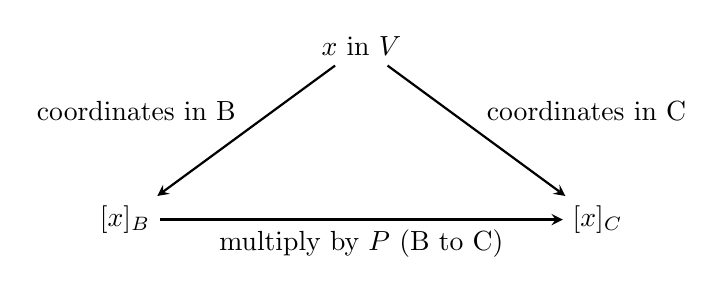
\begin{tikzpicture}[>=stealth,node distance=2.6cm]
  \node (x) at (3,2.2) {$x$ in $V$};
  \node (xb) at (0,0) {$[x]_B$};
  \node (xc) at (6,0) {$[x]_C$};
  \draw[->,thick] (x)--(xb) node[midway,above left] {coordinates in B};
  \draw[->,thick] (x)--(xc) node[midway,above right] {coordinates in C};
  \draw[->,thick] (xb)--(xc) node[midway,below] {multiply by $P$ (B to C)};
\end{tikzpicture}
\end{center}

\noindent\textbf{Figure 1.} Two sets of coordinates for one vector. Going down the left arrow and then across gives the same $\mathcal{C}$-coordinates as going down the right arrow directly (Theorem~\ref{thm:change}(a)).

\begin{think}{Expanding about a point}{taylorthink}
(a)~In Example~\ref{ex:taylor}, what does the coordinate vector $[p]_{\mathcal{B}}=(6,4,1)$ say about the value $p(1)$ and about $p'(1)$? (b)~Without any new computation, write down $P_{\mathcal{B}\leftarrow\mathcal{E}}$ for $\mathcal{B}=\{1,\ t-2,\ (t-2)^2\}$, by the same pattern as in the example, and say what its entries come from.
\end{think}

\begin{think}{Why the inverse exists}{whyinv}
(a)~Explain in one sentence why you can always return from $\mathcal{C}$-coordinates to $\mathcal{B}$-coordinates, and which matrix does it. (b)~In Theorem~\ref{thm:pcr}, which statement of Theorem~\ref{4.4-thm:PB} guarantees that $P_{\mathcal{C}}^{-1}$ exists? (c)~If $\mathcal{B}$ were the basis $\mathcal{B}=\{\bv{b}_2,\bv{b}_1\}$ (the same vectors in the other order), how would the columns of $P_{\mathcal{C}\leftarrow\mathcal{B}}$ change?
\end{think}

\begin{kc}{A change of basis in $\mathbb{P}_1$}{kcpoly}
In $\mathbb{P}_1$ let $\mathcal{E}=\{1,t\}$ and $\mathcal{B}=\{1+t,\ 1-t\}$. (a)~Find $P_{\mathcal{E}\leftarrow\mathcal{B}}$. (b)~Find $[p]_{\mathcal{B}}$ for $p(t)=5+3t$ by solving for it directly, and then check that $P_{\mathcal{E}\leftarrow\mathcal{B}}[p]_{\mathcal{B}}=[p]_{\mathcal{E}}$.
\end{kc}

% ---------------------------------------------------------------------
\subsection*{The matrix of a linear transformation}

Section~1.9 showed that every linear transformation $T:\R^n\to\R^m$ is multiplication by its standard matrix, whose columns are $T(\bv{e}_1),\dots,T(\bv{e}_n)$ (Theorem~\ref{1.9-thm:stdthm}). Those columns are the images of the standard basis, written in the standard basis of $\R^m$. We now allow any bases, and any vector spaces with coordinates. Let $T:V\to W$ be a linear transformation (Definition~\ref{4.2-def:lintrans}), let $\mathcal{B}=\{\bv{b}_1,\dots,\bv{b}_n\}$ be a basis of $V$ and let $\mathcal{C}$ be a basis of $W$ with $m$ vectors.

\begin{defn}{Matrix of a linear transformation}{mattrans}
The \emph{matrix of $T$ relative to $\mathcal{B}$ and $\mathcal{C}$} is the $m\times n$ matrix
\[
[T]_{\mathcal{C}\leftarrow\mathcal{B}}=\begin{bmatrix}[T(\bv{b}_1)]_{\mathcal{C}}&[T(\bv{b}_2)]_{\mathcal{C}}&\cdots&[T(\bv{b}_n)]_{\mathcal{C}}\end{bmatrix},
\]
whose $j$th column is the $\mathcal{C}$-coordinate vector of the image of the $j$th vector of $\mathcal{B}$. When $W=V$ and $\mathcal{C}=\mathcal{B}$, we write $[T]_{\mathcal{B}}$ and call it the \emph{$\mathcal{B}$-matrix of $T$}.
\end{defn}

\begin{thm}{The matrix does the work in coordinates}{matT}
For every $\bv{x}$ in $V$,
\[
[T(\bv{x})]_{\mathcal{C}}=[T]_{\mathcal{C}\leftarrow\mathcal{B}}\,[\bv{x}]_{\mathcal{B}}.
\]
\end{thm}

\begin{proof}
Write $\bv{x}=c_1\bv{b}_1+\cdots+c_n\bv{b}_n$. Because $T$ is linear (Theorem~\ref{4.2-thm:ltbasic}), $T(\bv{x})=c_1T(\bv{b}_1)+\cdots+c_nT(\bv{b}_n)$. The coordinate mapping into $\mathcal{C}$ is linear (Theorem~\ref{4.4-thm:coordmap}), so
\[
[T(\bv{x})]_{\mathcal{C}}=c_1[T(\bv{b}_1)]_{\mathcal{C}}+\cdots+c_n[T(\bv{b}_n)]_{\mathcal{C}}=[T]_{\mathcal{C}\leftarrow\mathcal{B}}\begin{bmatrix}c_1\\\vdots\\c_n\end{bmatrix}
\]
\end{proof}

So the recipe for building the matrix is also the reason it works: a linear transformation is determined by what it does to a basis, and the columns record exactly that.

\begin{proc}{Finding $[T]_{\mathcal{C}\leftarrow\mathcal{B}}$}{findM}
\begin{enumerate}[nosep]
  \item Compute $T(\bv{b}_j)$ for each vector of the basis $\mathcal{B}$ of the domain.
  \item Write each image in $\mathcal{C}$-coordinates (solve a system, or read off the coefficients).
  \item Put the coordinate vectors in the columns, in the order of $\mathcal{B}$.
  \item Check: take one $\bv{x}$ and compare $[T(\bv{x})]_{\mathcal{C}}$ with $[T]_{\mathcal{C}\leftarrow\mathcal{B}}[\bv{x}]_{\mathcal{B}}$.
\end{enumerate}
\end{proc}

\begin{exmp}{Differentiation from $\mathbb{P}_2$ to $\mathbb{P}_1$, with two bases}{deriv}
Let $T:\mathbb{P}_2\to\mathbb{P}_1$ be $T(p)=p'$. With $\mathcal{B}=\{1,t,t^2\}$ and $\mathcal{C}=\{1,t\}$: $T(1)=0$, $T(t)=1$, $T(t^2)=2t$, with $\mathcal{C}$-coordinates $(0,0)$, $(1,0)$, $(0,2)$. So
\[
[T]_{\mathcal{C}\leftarrow\mathcal{B}}=\begin{bmatrix}0&1&0\\0&0&2\end{bmatrix}.
\]
It is a $2\times3$ matrix: the domain has dimension $3$ and the codomain has dimension $2$. Now change the basis of the domain to $\mathcal{B}'=\{1,\ 1+t,\ 1+t+t^2\}$. The images are $T(1)=0$, $T(1+t)=1$ and $T(1+t+t^2)=1+2t$, with coordinates $(0,0)$, $(1,0)$, $(1,2)$, so
\[
[T]_{\mathcal{C}\leftarrow\mathcal{B}'}=\begin{bmatrix}0&1&1\\0&0&2\end{bmatrix}.
\]
Check with $p(t)=3+2t+t^2$. Then $[p]_{\mathcal{B}}=(3,2,1)$ and the first matrix gives $(2,2)$. In the basis $\mathcal{B}'$ we have $p=1\cdot1+1\cdot(1+t)+1\cdot(1+t+t^2)$, so $[p]_{\mathcal{B}'}=(1,1,1)$ and the second matrix gives $(0+1+1,\ 0+0+2)=(2,2)$. Both say $p'=2+2t$, which is $(2,2)$ in $\mathcal{C}$. \ $\checkmark$ The same transformation has two different matrices because the domain basis was changed.
\end{exmp}

\begin{exmp}{From $\R^2$ to $\R^3$ with nonstandard bases}{rtwothree}
Let $T:\R^2\to\R^3$ be $T(x_1,x_2)=(x_1+x_2,\ x_1-x_2,\ 2x_1)$. Take $\mathcal{B}=\{(1,1),(1,-1)\}$ and $\mathcal{C}=\{(1,0,0),(1,1,0),(1,1,1)\}$. Then $T(1,1)=(2,0,2)$ and $T(1,-1)=(0,2,2)$. To find their $\mathcal{C}$-coordinates, solve $a(1,0,0)+b(1,1,0)+c(1,1,1)$ from the bottom up: $c$ is the third entry, then $b+c$ is the second, then $a+b+c$ is the first. For $(2,0,2)$: $c=2$, $b=0-2=-2$, $a=2+2-2=2$. For $(0,2,2)$: $c=2$, $b=0$, $a=-2$. So
\[
[T]_{\mathcal{C}\leftarrow\mathcal{B}}=\begin{bmatrix}2&-2\\-2&0\\2&2\end{bmatrix}.
\]
Check with $\bv{x}=(3,1)$: $[\bv{x}]_{\mathcal{B}}=(2,1)$, and the matrix gives $(4-2,\ -4,\ 4+2)=(2,-4,6)$. Directly, $T(\bv{x})=(4,2,6)$ and $2(1,0,0)-4(1,1,0)+6(1,1,1)=(2-4+6,\ -4+6,\ 6)=(4,2,6)$. \ $\checkmark$
\end{exmp}

\begin{exmp}{The standard bases give the standard matrix}{stdcase}
For the same $T$ of Example~\ref{ex:rtwothree}, take the standard bases $\mathcal{E}_2$ of $\R^2$ and $\mathcal{E}_3$ of $\R^3$. Then $T(\bv{e}_1)=(1,1,2)$ and $T(\bv{e}_2)=(1,-1,0)$ are already their own coordinate vectors, so $[T]_{\mathcal{E}_3\leftarrow\mathcal{E}_2}=\begin{bmatrix}1&1\\1&-1\\2&0\end{bmatrix}$, the standard matrix of Section~1.9. In general the standard matrix is the matrix of $T$ relative to the standard bases. Compare the two matrices for $T$: the standard one uses the easiest bases, and the one in Example~\ref{ex:rtwothree} uses bases chosen for another reason; each is correct for its own bases.
\end{exmp}

\begin{think}{Sizes and the standard bases}{sizes}
(a)~What is the size of $[T]_{\mathcal{C}\leftarrow\mathcal{B}}$ if $\dim V=4$ and $\dim W=2$, and what does the size say about the domain and the codomain? (b)~If $\mathcal{B}$ is any basis of $\R^n$ and $\mathcal{E}$ is the standard basis, what is $P_{\mathcal{E}\leftarrow\mathcal{B}}$, and why? (c)~Why do we need the same basis on both sides, and not just two bases of the same space, before we can call the matrix $[T]_{\mathcal{B}}$?
\end{think}

\begin{kc}{The matrix of multiplication by $t$}{kcmat}
Let $T:\mathbb{P}_1\to\mathbb{P}_2$ be $T(p)(t)=t\,p(t)$, with the bases $\{1,t\}$ and $\{1,t,t^2\}$. (a)~Find the matrix of $T$. (b)~Use it to find $T(4-3t)$ in coordinates, and check by multiplying out.
\end{kc}

% ---------------------------------------------------------------------
\subsection*{One transformation, two bases}

When the domain and the codomain are the same space and we use one basis for both, we get a square matrix $[T]_{\mathcal{B}}$. Different bases give different square matrices. How are they related? The change-of-basis matrix is the link.

\begin{thm}{Two matrices of one transformation}{similarmatrices}
Let $T:V\to V$ be a linear transformation, let $\mathcal{B}$ and $\mathcal{C}$ be bases of $V$ and let $P=P_{\mathcal{B}\leftarrow\mathcal{C}}$. Then
\[
[T]_{\mathcal{C}}=P^{-1}\,[T]_{\mathcal{B}}\,P.
\]
In particular, for the transformation $T(\bv{x})=A\bv{x}$ of $\R^n$ and a basis $\mathcal{B}$ of $\R^n$,
\[
[T]_{\mathcal{B}}=P_{\mathcal{B}}^{-1}AP_{\mathcal{B}}.
\]
\end{thm}

\begin{proof}
By Theorem~\ref{thm:change}, $P^{-1}=P_{\mathcal{C}\leftarrow\mathcal{B}}$. For every $\bv{x}$ in $V$, using Theorem~\ref{thm:change}(a) and Theorem~\ref{thm:matT},
\[
[T(\bv{x})]_{\mathcal{C}}=P_{\mathcal{C}\leftarrow\mathcal{B}}\,[T(\bv{x})]_{\mathcal{B}}=P^{-1}[T]_{\mathcal{B}}\,[\bv{x}]_{\mathcal{B}}=P^{-1}[T]_{\mathcal{B}}\,P\,[\bv{x}]_{\mathcal{C}}.
\]
Also $[T(\bv{x})]_{\mathcal{C}}=[T]_{\mathcal{C}}[\bv{x}]_{\mathcal{C}}$ by Theorem~\ref{thm:matT}. So the matrices $[T]_{\mathcal{C}}$ and $P^{-1}[T]_{\mathcal{B}}P$ have the same effect on every coordinate vector $[\bv{x}]_{\mathcal{C}}$. Taking $\bv{x}=\bv{c}_j$, whose coordinate vector is $\bv{e}_j$, shows that their $j$th columns agree, so the matrices are equal.

For the second statement, take $V=\R^n$, let $\mathcal{E}$ be the standard basis and $\mathcal{B}$ any basis. The standard matrix $A$ is $[T]_{\mathcal{E}}$ (Example~\ref{ex:stdcase}), and $P_{\mathcal{E}\leftarrow\mathcal{B}}=P_{\mathcal{B}}$ because the standard coordinates of $\bv{b}_j$ are $\bv{b}_j$ itself. Apply the first statement with the roles $\mathcal{B}\to\mathcal{E}$ and $\mathcal{C}\to\mathcal{B}$: $P=P_{\mathcal{E}\leftarrow\mathcal{B}}=P_{\mathcal{B}}$ and $[T]_{\mathcal{B}}=P_{\mathcal{B}}^{-1}AP_{\mathcal{B}}$.
\end{proof}

\begin{exmp}{The $\mathcal{B}$-matrix of $\bv{x}\mapsto A\bv{x}$}{bmat}
Let $A=\begin{bmatrix}7&2\\-4&1\end{bmatrix}$, $T(\bv{x})=A\bv{x}$ and $\mathcal{B}=\{(1,0),(1,1)\}$. \emph{By the definition.} $T(\bv{b}_1)=(7,-4)$ and $T(\bv{b}_2)=(9,-3)$. Solving $a(1,0)+b(1,1)$ for each: $(7,-4)=11\bv{b}_1-4\bv{b}_2$ and $(9,-3)=12\bv{b}_1-3\bv{b}_2$. So $[T]_{\mathcal{B}}=\begin{bmatrix}11&12\\-4&-3\end{bmatrix}$. \emph{By Theorem~\ref{thm:similarmatrices}.} $P_{\mathcal{B}}=\begin{bmatrix}1&1\\0&1\end{bmatrix}$ and $P_{\mathcal{B}}^{-1}=\begin{bmatrix}1&-1\\0&1\end{bmatrix}$, so
\[
P_{\mathcal{B}}^{-1}AP_{\mathcal{B}}=\begin{bmatrix}1&-1\\0&1\end{bmatrix}\begin{bmatrix}7&9\\-4&-3\end{bmatrix}=\begin{bmatrix}11&12\\-4&-3\end{bmatrix},
\]
the same matrix. Check with $\bv{x}=(3,1)$: $[\bv{x}]_{\mathcal{B}}=(2,1)$ and $[T]_{\mathcal{B}}(2,1)=(34,-11)$, while $A\bv{x}=(23,-11)$ has $\mathcal{B}$-coordinates $(23+11,\ -11)=(34,-11)$. \ $\checkmark$
\end{exmp}

\begin{exmp}{The same transformation in a second basis}{twomats}
Keep $T(\bv{x})=A\bv{x}$ with $A=\begin{bmatrix}7&2\\-4&1\end{bmatrix}$, and let $\mathcal{B}=\{(1,0),(1,1)\}$ as above and $\mathcal{C}=\{(1,-2),(1,-1)\}$. We write the vectors of $\mathcal{C}$ in $\mathcal{B}$-coordinates: $(1,-2)=3(1,0)-2(1,1)$ and $(1,-1)=2(1,0)-1(1,1)$, so $P=P_{\mathcal{B}\leftarrow\mathcal{C}}=\begin{bmatrix}3&2\\-2&-1\end{bmatrix}$ and $P^{-1}=\begin{bmatrix}-1&-2\\2&3\end{bmatrix}$. By Theorem~\ref{thm:similarmatrices},
\[
[T]_{\mathcal{C}}=P^{-1}[T]_{\mathcal{B}}P=\begin{bmatrix}-1&-2\\2&3\end{bmatrix}\begin{bmatrix}11&12\\-4&-3\end{bmatrix}\begin{bmatrix}3&2\\-2&-1\end{bmatrix}=\begin{bmatrix}-3&-6\\10&15\end{bmatrix}\begin{bmatrix}3&2\\-2&-1\end{bmatrix}=\begin{bmatrix}3&0\\0&5\end{bmatrix}.
\]
The matrix in the second basis is diagonal, which the matrix in the first basis was not. Directly: $A(1,-2)=(3,-6)=3(1,-2)$ and $A(1,-1)=(5,-5)=5(1,-1)$, so the columns of $[T]_{\mathcal{C}}$ are $(3,0)$ and $(0,5)$. \ $\checkmark$ One transformation, two matrices, and one of them is much nicer.
\end{exmp}

\begin{think}{The identity transformation}{ident}
(a)~What is $[T]_{\mathcal{B}}$ when $T$ is the identity transformation $T(\bv{x})=\bv{x}$, for any basis $\mathcal{B}$? (b)~Check that Theorem~\ref{thm:similarmatrices} agrees: what does it give for $[T]_{\mathcal{C}}$? (c)~What is $[T]_{\mathcal{B}}$ for $T(\bv{x})=3\bv{x}$ in every basis?
\end{think}

\begin{kc}{A $\mathcal{B}$-matrix}{kcbm}
Let $A=\begin{bmatrix}3&1\\0&2\end{bmatrix}$, $T(\bv{x})=A\bv{x}$ and $\mathcal{B}=\{(1,0),(1,1)\}$. (a)~Find $[T]_{\mathcal{B}}$ from the definition, by finding the $\mathcal{B}$-coordinates of $T(\bv{b}_1)$ and $T(\bv{b}_2)$. (b)~Confirm it with $P_{\mathcal{B}}^{-1}AP_{\mathcal{B}}$.
\end{kc}

% ---------------------------------------------------------------------
\subsection*{The diagonal case}

The matrix $[T]_{\mathcal{B}}$ is easiest to understand when it is diagonal. In Example~\ref{ex:twomats} the basis $\mathcal{C}$ made $[T]_{\mathcal{C}}$ diagonal, with entries $3$ and $5$. What does the transformation do?

\begin{thm}{The diagonal case}{diagcase}
Let $T:V\to V$ be a linear transformation and let $\mathcal{B}=\{\bv{b}_1,\dots,\bv{b}_n\}$ be a basis of $V$. Then $[T]_{\mathcal{B}}$ is a diagonal matrix with diagonal entries $d_1,\dots,d_n$ if and only if
\[
T(\bv{b}_j)=d_j\,\bv{b}_j\qquad\text{for each }j=1,\dots,n.
\]
In that case $T(c_1\bv{b}_1+\cdots+c_n\bv{b}_n)=d_1c_1\bv{b}_1+\cdots+d_nc_n\bv{b}_n$: $T$ scales the coordinate along each basis vector by its own number.
\end{thm}

\begin{proof}
The $j$th column of $[T]_{\mathcal{B}}$ is $[T(\bv{b}_j)]_{\mathcal{B}}$. The matrix is diagonal with entries $d_j$ exactly when this column is $d_j\bv{e}_j$ for every $j$. A vector has $\mathcal{B}$-coordinate vector $d_j\bv{e}_j$ exactly when it equals $d_j\bv{b}_j$, because coordinates relative to a basis are unique (Theorem~\ref{4.4-thm:unique}). So the matrix is diagonal with entries $d_j$ if and only if $T(\bv{b}_j)=d_j\bv{b}_j$ for all $j$. The last formula follows from linearity: $T(\sum c_j\bv{b}_j)=\sum c_jT(\bv{b}_j)=\sum c_jd_j\bv{b}_j$.
\end{proof}

\begin{exmp}{A transformation that scales two directions}{scales}
In Example~\ref{ex:twomats} the basis is $\mathcal{C}=\{\bv{c}_1,\bv{c}_2\}=\{(1,-2),(1,-1)\}$ and $A=\begin{bmatrix}7&2\\-4&1\end{bmatrix}$. By Theorem~\ref{thm:diagcase}, $T(\bv{c}_1)=3\bv{c}_1$ and $T(\bv{c}_2)=5\bv{c}_2$, as we checked. So $T$ stretches the line through $\bv{c}_1$ by the factor $3$ and the line through $\bv{c}_2$ by the factor $5$. To compute $T(\bv{x})$ for $\bv{x}=(3,1)$, find $[\bv{x}]_{\mathcal{C}}$: $a(1,-2)+b(1,-1)=(3,1)$ gives $a+b=3$ and $-2a-b=1$, so $a=-4$ and $b=7$. Then $T(\bv{x})=3(-4)\bv{c}_1+5(7)\bv{c}_2=-12(1,-2)+35(1,-1)=(23,-11)$, and directly $A\bv{x}=(21+2,\ -12+1)=(23,-11)$. \ $\checkmark$
\end{exmp}

\begin{center}
\begin{tikzpicture}[>=stealth,scale=1.1]
  \draw[gray!50,->] (-1.2,0)--(6.8,0) node[right] {line of c1};
  \draw[gray!50,->] (-0.5,-0.2)--(0.9,3.2) node[above] {line of c2};
  \draw[->,thick] (0,0)--(1.5,0) node[below] {c1};
  \draw[->,thick] (0,0)--(0.25,0.6) node[left] {c2};
  \draw[->,thick,blue] (0,0)--(1.75,0.6) node[above right] {x};
  \draw[->,thick,red] (0,0)--(4.5,3.0) node[above right] {T(x)};
  \draw[dashed] (1.5,0)--(1.75,0.6);
  \draw[dashed] (0.25,0.6)--(1.75,0.6);
\end{tikzpicture}
\end{center}

\noindent\textbf{Figure 2.} A schematic picture of the diagonal case. The vector $\bv{x}=\bv{c}_1+\bv{c}_2$ is shown as the diagonal of the parallelogram on the two basis vectors. The image has the same description with each side stretched by its own factor, here $3$ for the first side and $5$ for the second. The drawing is not to scale.

\begin{exmp}{Building a transformation from a diagonal matrix}{buildA}
Let $\mathcal{B}=\{(1,0,0),(1,1,0),(1,1,1)\}$. Find the standard matrix $A$ of the transformation $T$ of $\R^3$ with $[T]_{\mathcal{B}}=D=\operatorname{diag}(2,-1,4)$. By Theorem~\ref{thm:similarmatrices}, $D=P_{\mathcal{B}}^{-1}AP_{\mathcal{B}}$, so $A=P_{\mathcal{B}}DP_{\mathcal{B}}^{-1}$ with $P_{\mathcal{B}}=\begin{bmatrix}1&1&1\\0&1&1\\0&0&1\end{bmatrix}$ and $P_{\mathcal{B}}^{-1}=\begin{bmatrix}1&-1&0\\0&1&-1\\0&0&1\end{bmatrix}$. Then
\[
A=\begin{bmatrix}2&-1&4\\0&-1&4\\0&0&4\end{bmatrix}\begin{bmatrix}1&-1&0\\0&1&-1\\0&0&1\end{bmatrix}=\begin{bmatrix}2&-3&5\\0&-1&5\\0&0&4\end{bmatrix}.
\]
Check with Theorem~\ref{thm:diagcase}: $A(1,0,0)=(2,0,0)=2\bv{b}_1$, $A(1,1,0)=(2-3,\ -1,\ 0)=(-1,-1,0)=-\bv{b}_2$ and $A(1,1,1)=(4,4,4)=4\bv{b}_3$. \ $\checkmark$
\end{exmp}

\begin{exmp}{Finding a basis that makes a transformation diagonal}{findbasis}
Let $T(\bv{x})=A\bv{x}$ with $A=\begin{bmatrix}5&-4\\2&-1\end{bmatrix}$. Suppose we are told that $T$ scales some nonzero vector by the factor $1$ and another by the factor $3$. By Theorem~\ref{thm:diagcase} such vectors, if they form a basis, give a diagonal matrix. We find them by solving $A\bv{b}=d\bv{b}$, that is, $(A-dI)\bv{b}=\bv{0}$. For $d=1$: $A-I=\begin{bmatrix}4&-4\\2&-2\end{bmatrix}$ gives $b_1=b_2$, so $\bv{b}_1=(1,1)$. For $d=3$: $A-3I=\begin{bmatrix}2&-4\\2&-4\end{bmatrix}$ gives $b_1=2b_2$, so $\bv{b}_2=(2,1)$. The two vectors are independent (neither is a multiple of the other), so $\mathcal{B}=\{(1,1),(2,1)\}$ is a basis of $\R^2$, and $T(\bv{b}_1)=A(1,1)=(1,1)$ and $T(\bv{b}_2)=A(2,1)=(6,3)=3\bv{b}_2$. Therefore $[T]_{\mathcal{B}}=\begin{bmatrix}1&0\\0&3\end{bmatrix}$. Check: $P_{\mathcal{B}}^{-1}AP_{\mathcal{B}}=\begin{bmatrix}-1&2\\1&-1\end{bmatrix}\begin{bmatrix}1&6\\1&3\end{bmatrix}=\begin{bmatrix}1&0\\0&3\end{bmatrix}$. \ $\checkmark$
\end{exmp}

\begin{exmp}{Diagonal in the standard basis of $\mathbb{P}_2$}{polydiag}
Let $T:\mathbb{P}_2\to\mathbb{P}_2$ be $T(p)(t)=p(-t)$. Then $T(1)=1$, $T(t)=-t$ and $T(t^2)=t^2$, so $T$ scales each vector of $\mathcal{E}=\{1,t,t^2\}$: by $1$, by $-1$ and by $1$. By Theorem~\ref{thm:diagcase}, $[T]_{\mathcal{E}}=\operatorname{diag}(1,-1,1)$. For another transformation, $S(p)(t)=t\,p'(t)$, we get $S(1)=0$, $S(t)=t$ and $S(t^2)=2t^2$, so $[S]_{\mathcal{E}}=\operatorname{diag}(0,1,2)$. In coordinates, $T$ changes the sign of the coefficient of $t$, and $S$ multiplies the coefficient of $t^k$ by $k$.
\end{exmp}

\begin{exmp}{A transformation with no such basis}{norot}
Let $T(\bv{x})=A\bv{x}$ with $A=\begin{bmatrix}0&-1\\1&0\end{bmatrix}$, the rotation by a quarter turn. Suppose $T(\bv{b})=d\bv{b}$ for a nonzero $\bv{b}=(b_1,b_2)$ and a real number $d$. Then $(-b_2,b_1)=(db_1,db_2)$, so $-b_2=db_1$ and $b_1=db_2$. Substituting the second into the first gives $-b_2=d^2b_2$, that is, $(1+d^2)b_2=0$. Since $1+d^2\neq0$, $b_2=0$ and then $b_1=db_2=0$, a contradiction. So no nonzero real vector is merely scaled by $T$, and no basis of $\R^2$ makes $[T]_{\mathcal{B}}$ diagonal. The diagonal case does not always exist.
\end{exmp}

\begin{think}{What a diagonal matrix says}{scaledline}
(a)~In Example~\ref{ex:scales}, what does $T$ do to every vector on the line through $\bv{c}_2$? (b)~If $[T]_{\mathcal{B}}=\operatorname{diag}(2,0)$, what does $T$ do to $\bv{b}_2$, and which vectors does $T$ send to $\bv{0}$? (c)~In Example~\ref{ex:norot}, which geometric fact explains why no direction is merely scaled?
\end{think}

\begin{kc}{Is the matrix diagonal?}{kcdiag}
Let $A=\begin{bmatrix}0&1\\1&0\end{bmatrix}$ and $T(\bv{x})=A\bv{x}$. (a)~Is $[T]_{\mathcal{B}}$ diagonal for $\mathcal{B}=\{(1,1),(1,-1)\}$? If so, what are its entries? (b)~Is it diagonal for $\mathcal{B}'=\{(1,0),(1,1)\}$?
\end{kc}

\noindent\textbf{A remark on names.} A nonzero vector that a transformation merely scales, as the basis vectors $\bv{b}_j$ are in Theorem~\ref{thm:diagcase}, is called an eigenvector of the transformation, and the factor $d_j$ by which it is scaled is called its eigenvalue. The sections on eigenvectors and diagonalization that come before this one study when such a basis exists and how to find it; here we only observed what a diagonal matrix of a transformation means.

\begin{kc}{True or false?}{kctf}
Justify each answer. (a)~$P_{\mathcal{C}\leftarrow\mathcal{B}}=P_{\mathcal{B}\leftarrow\mathcal{C}}$. (b)~$P_{\mathcal{C}\leftarrow\mathcal{B}}$ is always an invertible matrix. (c)~If $T:\R^3\to\R^2$ is linear, every matrix of $T$ relative to a basis of $\R^3$ and a basis of $\R^2$ has $2$ rows and $3$ columns. (d)~If $[T]_{\mathcal{B}}$ is diagonal for one basis $\mathcal{B}$, it is diagonal for every basis. (e)~Reordering the vectors of $\mathcal{B}$ changes $[T]_{\mathcal{B}}$ in general. (f)~If $T$ is the zero transformation then $[T]_{\mathcal{C}\leftarrow\mathcal{B}}$ is the zero matrix for all bases.
\end{kc}

\begin{think}{Reordering and the standard matrix}{reorder}
(a)~If we swap the two basis vectors of $\mathcal{B}=\{\bv{b}_1,\bv{b}_2\}$, what happens to the columns of $[T]_{\mathcal{B}}$, and what happens to its rows? (b)~Which matrix, for the same $T$, is more natural to call ``the'' matrix of $T$: the standard matrix, or $[T]_{\mathcal{B}}$? Why is the standard one given a special name?
\end{think}

\subsection*{Summary}
\begin{itemize}
  \item \textbf{Change of basis.} $P_{\mathcal{C}\leftarrow\mathcal{B}}$ has the columns $[\bv{b}_j]_{\mathcal{C}}$, and $[\bv{x}]_{\mathcal{C}}=P_{\mathcal{C}\leftarrow\mathcal{B}}[\bv{x}]_{\mathcal{B}}$. It is invertible with inverse $P_{\mathcal{B}\leftarrow\mathcal{C}}$ (Theorem~\ref{thm:change}). In $\R^n$ it is $P_{\mathcal{C}}^{-1}P_{\mathcal{B}}$, found by row reducing $[\,P_{\mathcal{C}}\ \ P_{\mathcal{B}}\,]$ (Theorem~\ref{thm:pcr}, Procedure~\ref{proc:findp}).
  \item \textbf{Matrix of a transformation.} $[T]_{\mathcal{C}\leftarrow\mathcal{B}}$ has the columns $[T(\bv{b}_j)]_{\mathcal{C}}$, and $[T(\bv{x})]_{\mathcal{C}}=[T]_{\mathcal{C}\leftarrow\mathcal{B}}[\bv{x}]_{\mathcal{B}}$ (Definition~\ref{def:mattrans}, Theorem~\ref{thm:matT}). With the standard bases it is the standard matrix.
  \item \textbf{Two bases.} $[T]_{\mathcal{C}}=P^{-1}[T]_{\mathcal{B}}P$ with $P=P_{\mathcal{B}\leftarrow\mathcal{C}}$, and $[T]_{\mathcal{B}}=P_{\mathcal{B}}^{-1}AP_{\mathcal{B}}$ for $\bv{x}\mapsto A\bv{x}$ (Theorem~\ref{thm:similarmatrices}).
  \item \textbf{Diagonal case.} $[T]_{\mathcal{B}}$ is diagonal exactly when $T$ scales each basis vector (Theorem~\ref{thm:diagcase}). Such a basis does not always exist (Example~\ref{ex:norot}).
\end{itemize}

\subsection*{Questions to think about before the next section}
\begin{enumerate}[nosep]
  \item Let $T$ be the identity transformation of $V$. What is $[T]_{\mathcal{C}\leftarrow\mathcal{B}}$ for two different bases $\mathcal{B}$ and $\mathcal{C}$?
  \item Suppose $S$ and $T$ are linear transformations $V\to W$ with $[S]_{\mathcal{C}\leftarrow\mathcal{B}}=[T]_{\mathcal{C}\leftarrow\mathcal{B}}$ for some bases. Must $S=T$?
  \item Is every invertible $n\times n$ matrix the change-of-basis matrix between two bases of $\R^n$?
\end{enumerate}

\subsection*{Example bank}
The twelve examples below add problem types that the worked examples above do not cover: changing coordinates between bases of $\R^2$, $\R^3$ and $\mathbb{P}_2$; matrices of transformations between different spaces and with two different bases; $\mathcal{B}$-matrices and the diagonal case, including a $3\times3$ case and the reverse problem of building the transformation; reading information from a diagonal matrix; and three proofs. Within each group the examples go from easier to harder. Work each problem before you read its solution.

\textbf{What is in this bank.}
\begin{itemize}
  \item \textbf{Bank A, change of basis:} Example~\ref{ex:b-r2} (row reducing in $\R^2$, both directions), Example~\ref{ex:b-r3} (an $\R^3$ case by solving from the bottom up) and Example~\ref{ex:b-poly} (a basis of $\mathbb{P}_2$).
  \item \textbf{Bank B, matrix of a transformation:} Example~\ref{ex:b-ev} (from $\mathbb{P}_2$ to $\R^2$, with the standard and a second basis) and Example~\ref{ex:b-two} ($\R^2$ to $\R^2$ with a different basis on each side).
  \item \textbf{Bank C, $\mathcal{B}$-matrices and the diagonal case:} Example~\ref{ex:b-tri} (a triangular $\mathcal{B}$-matrix), Example~\ref{ex:b-three} (a $3\times3$ basis with a diagonal matrix) and Example~\ref{ex:b-build} (from a diagonal matrix back to $A$).
  \item \textbf{Bank D, reading a diagonal matrix:} Example~\ref{ex:b-read} (kernel, range and an image from $\operatorname{diag}(2,0,5)$).
  \item \textbf{Bank E, proofs:} Example~\ref{ex:b-pid} (beginner: $P_{\mathcal{C}\leftarrow\mathcal{B}}=I$), Example~\ref{ex:b-chain} (intermediate: composing changes of basis) and Example~\ref{ex:b-invert} (intermediate: invertibility of $A$ and of $[T]_{\mathcal{B}}$).
\end{itemize}

\subsection*{Bank A: Change of basis}
\begin{exmp}{Row reducing in $\R^2$, both directions}{b-r2}
Let $\mathcal{B}=\{(1,3),(2,5)\}$ and $\mathcal{C}=\{(2,1),(3,2)\}$. Find $P_{\mathcal{C}\leftarrow\mathcal{B}}$ and $P_{\mathcal{B}\leftarrow\mathcal{C}}$, and check them on $\bv{x}=(5,9)$.

\textbf{Solution.} Row reduce $[\,P_{\mathcal{C}}\ \ P_{\mathcal{B}}\,]$ (Theorem~\ref{thm:pcr}):
\begin{align*}
\begin{amat}{cc|cc}2 & 3 & 1 & 2\\1 & 2 & 3 & 5\end{amat}
&\rops{R_1\leftrightarrow R_2}
\begin{amat}{cc|cc}1 & 2 & 3 & 5\\2 & 3 & 1 & 2\end{amat}
\rops{R_2-2R_1}
\begin{amat}{cc|cc}1 & 2 & 3 & 5\\0 & -1 & -5 & -8\end{amat}
\\[4pt]
&\rops{-R_2}
\begin{amat}{cc|cc}1 & 2 & 3 & 5\\0 & 1 & 5 & 8\end{amat}
\rops{R_1-2R_2}
\begin{amat}{cc|cc}1 & 0 & -7 & -11\\0 & 1 & 5 & 8\end{amat}
\end{align*}
so $P_{\mathcal{C}\leftarrow\mathcal{B}}=\begin{bmatrix}-7&-11\\5&8\end{bmatrix}$. Its determinant is $-56+55=-1$, so $P_{\mathcal{B}\leftarrow\mathcal{C}}$ is its inverse (Theorem~\ref{thm:change}(b)): $P_{\mathcal{B}\leftarrow\mathcal{C}}=\begin{bmatrix}-8&-11\\5&7\end{bmatrix}$. Check the product: $\begin{bmatrix}-7&-11\\5&8\end{bmatrix}\begin{bmatrix}-8&-11\\5&7\end{bmatrix}=\begin{bmatrix}56-55&77-77\\-40+40&-55+56\end{bmatrix}=I$. Directly, $[\bv{x}]_{\mathcal{B}}=(-7,6)$ since $-7(1,3)+6(2,5)=(5,9)$, and $[\bv{x}]_{\mathcal{C}}=(-17,13)$ since $-17(2,1)+13(3,2)=(5,9)$. The matrix gives $\begin{bmatrix}-7&-11\\5&8\end{bmatrix}\begin{bmatrix}-7\\6\end{bmatrix}=\begin{bmatrix}49-66\\-35+48\end{bmatrix}=\begin{bmatrix}-17\\13\end{bmatrix}$. \ $\checkmark$
\end{exmp}

\begin{exmp}{An $\R^3$ case by solving from the bottom up}{b-r3}
Let $\mathcal{B}=\{(1,1,0),(0,1,1),(0,0,1)\}$ and $\mathcal{C}=\{(1,0,0),(1,1,0),(1,1,1)\}$. Find $P_{\mathcal{C}\leftarrow\mathcal{B}}$ without row reducing.

\textbf{Solution.} The vectors of $\mathcal{C}$ are triangular, so each $\mathcal{C}$-coordinate vector can be read off from the bottom: for $(x_1,x_2,x_3)=a\bv{c}_1+b\bv{c}_2+c\bv{c}_3$ we get $c=x_3$, then $b=x_2-x_3$, then $a=x_1-x_2$. Apply this to each vector of $\mathcal{B}$: $(1,1,0)$ gives $c=0$, $b=1$, $a=0$; $(0,1,1)$ gives $c=1$, $b=0$, $a=-1$; $(0,0,1)$ gives $c=1$, $b=-1$, $a=0$. So
\[
P_{\mathcal{C}\leftarrow\mathcal{B}}=\begin{bmatrix}0&-1&0\\1&0&-1\\0&1&1\end{bmatrix}.
\]
Check with $\bv{x}=(2,3,1)$: $[\bv{x}]_{\mathcal{B}}=(2,1,0)$ since $2(1,1,0)+1(0,1,1)=(2,3,1)$, and $[\bv{x}]_{\mathcal{C}}$ from the rule is $c=1$, $b=2$, $a=-1$, that is $(-1,2,1)$. The matrix gives $(0-1+0,\ 2+0-0,\ 0+1+0)=(-1,2,1)$. \ $\checkmark$
\end{exmp}

\begin{exmp}{A basis of $\mathbb{P}_2$}{b-poly}
Let $\mathcal{E}=\{1,t,t^2\}$ and $\mathcal{B}=\{1,\ 1+t,\ t+t^2\}$. Find $P_{\mathcal{E}\leftarrow\mathcal{B}}$ and $P_{\mathcal{B}\leftarrow\mathcal{E}}$, and write $p(t)=2-t+3t^2$ in the basis $\mathcal{B}$.

\textbf{Solution.} The $\mathcal{E}$-coordinates of the vectors of $\mathcal{B}$ are $(1,0,0)$, $(1,1,0)$, $(0,1,1)$, so $P_{\mathcal{E}\leftarrow\mathcal{B}}=\begin{bmatrix}1&1&0\\0&1&1\\0&0&1\end{bmatrix}$. For the inverse, express $1$, $t$ and $t^2$ through $\mathcal{B}$: $1=1$; $t=(1+t)-1$; $t^2=(t+t^2)-t=(t+t^2)-(1+t)+1$. So $P_{\mathcal{B}\leftarrow\mathcal{E}}=\begin{bmatrix}1&-1&1\\0&1&-1\\0&0&1\end{bmatrix}$, and $\begin{bmatrix}1&1&0\\0&1&1\\0&0&1\end{bmatrix}\begin{bmatrix}1&-1&1\\0&1&-1\\0&0&1\end{bmatrix}=I$. Then $[p]_{\mathcal{E}}=(2,-1,3)$ and
\[
[p]_{\mathcal{B}}=P_{\mathcal{B}\leftarrow\mathcal{E}}[p]_{\mathcal{E}}=\begin{bmatrix}1&-1&1\\0&1&-1\\0&0&1\end{bmatrix}\begin{bmatrix}2\\-1\\3\end{bmatrix}=\begin{bmatrix}6\\-4\\3\end{bmatrix}.
\]
Check: $6\cdot1-4(1+t)+3(t+t^2)=6-4-4t+3t+3t^2=2-t+3t^2$. \ $\checkmark$
\end{exmp}

\subsection*{Bank B: The matrix of a transformation}
\begin{exmp}{From $\mathbb{P}_2$ to $\R^2$, with two bases of $\mathbb{P}_2$}{b-ev}
Let $T:\mathbb{P}_2\to\R^2$ be $T(p)=(p(0),\,p(1))$. Find the matrix of $T$ relative to $\mathcal{E}=\{1,t,t^2\}$ and the standard basis of $\R^2$, and then relative to $\mathcal{B}=\{1,\ t-1,\ (t-1)^2\}$ and the standard basis. Explain how the two are related.

\textbf{Solution.} For $\mathcal{E}$: $T(1)=(1,1)$, $T(t)=(0,1)$, $T(t^2)=(0,1)$, so $M_{\mathcal{E}}=\begin{bmatrix}1&0&0\\1&1&1\end{bmatrix}$. For $\mathcal{B}$: $T(1)=(1,1)$, $T(t-1)=(-1,0)$ and $T\bigl((t-1)^2\bigr)=(1,0)$, since $(0-1)^2=1$ and $(1-1)^2=0$; so $M_{\mathcal{B}}=\begin{bmatrix}1&-1&1\\1&0&0\end{bmatrix}$. The relation: by Theorem~\ref{thm:matT} and Theorem~\ref{thm:change}, $T(p)$ in $\R^2$ equals $M_{\mathcal{E}}[p]_{\mathcal{E}}$ and also $M_{\mathcal{B}}[p]_{\mathcal{B}}$, and $[p]_{\mathcal{E}}=P_{\mathcal{E}\leftarrow\mathcal{B}}[p]_{\mathcal{B}}$, so $M_{\mathcal{B}}=M_{\mathcal{E}}P_{\mathcal{E}\leftarrow\mathcal{B}}$. With $P_{\mathcal{E}\leftarrow\mathcal{B}}=\begin{bmatrix}1&-1&1\\0&1&-2\\0&0&1\end{bmatrix}$ from Example~\ref{ex:taylor}:
\[
M_{\mathcal{E}}P_{\mathcal{E}\leftarrow\mathcal{B}}=\begin{bmatrix}1&0&0\\1&1&1\end{bmatrix}\begin{bmatrix}1&-1&1\\0&1&-2\\0&0&1\end{bmatrix}=\begin{bmatrix}1&-1&1\\1&0&0\end{bmatrix}=M_{\mathcal{B}}.
\]
Check with $p(t)=3+2t+t^2$, where $[p]_{\mathcal{B}}=(6,4,1)$: $M_{\mathcal{B}}(6,4,1)=(6-4+1,\ 6)=(3,6)$, and directly $(p(0),p(1))=(3,6)$. \ $\checkmark$
\end{exmp}

\begin{exmp}{A different basis on each side}{b-two}
Let $T(\bv{x})=A\bv{x}$ with $A=\begin{bmatrix}2&1\\3&2\end{bmatrix}$, and take $\mathcal{B}=\{(1,1),(1,2)\}$ as the basis of the domain and $\mathcal{C}=\{(1,0),(1,1)\}$ as the basis of the codomain. Find $[T]_{\mathcal{C}\leftarrow\mathcal{B}}$ and check it.

\textbf{Solution.} $T(1,1)=(3,5)$ and $T(1,2)=(4,7)$. Write each in $\mathcal{C}$: $(x_1,x_2)=a(1,0)+b(1,1)$ gives $b=x_2$ and $a=x_1-x_2$. So $(3,5)$ has coordinates $(-2,5)$ and $(4,7)$ has coordinates $(-3,7)$, and
\[
[T]_{\mathcal{C}\leftarrow\mathcal{B}}=\begin{bmatrix}-2&-3\\5&7\end{bmatrix}.
\]
Check with $\bv{x}=(3,5)$: $[\bv{x}]_{\mathcal{B}}=(1,2)$ and the matrix gives $(-2-6,\ 5+14)=(-8,19)$. Directly $T(\bv{x})=(11,19)$, which has $\mathcal{C}$-coordinates $(11-19,\ 19)=(-8,19)$. \ $\checkmark$ Note that the two bases are different, so this is not a $\mathcal{B}$-matrix and Theorem~\ref{thm:similarmatrices} does not apply to it.
\end{exmp}

\subsection*{Bank C: $\mathcal{B}$-matrices and the diagonal case}
\begin{exmp}{A triangular $\mathcal{B}$-matrix}{b-tri}
Let $A=\begin{bmatrix}6&-2\\3&1\end{bmatrix}$, $T(\bv{x})=A\bv{x}$ and $\mathcal{B}=\{(1,1),(1,2)\}$. Find $[T]_{\mathcal{B}}$, and say what its first column says about $T$.

\textbf{Solution.} $T(\bv{b}_1)=A(1,1)=(4,4)=4\bv{b}_1$. $T(\bv{b}_2)=A(1,2)=(2,5)$, and $a(1,1)+b(1,2)=(2,5)$ gives $a+2b=5$ and $a+b=2$, so $b=3$ and $a=-1$: $T(\bv{b}_2)=-\bv{b}_1+3\bv{b}_2$. So
\[
[T]_{\mathcal{B}}=\begin{bmatrix}4&-1\\0&3\end{bmatrix}.
\]
Check by Theorem~\ref{thm:similarmatrices}: $P_{\mathcal{B}}^{-1}=\begin{bmatrix}2&-1\\-1&1\end{bmatrix}$ and $AP_{\mathcal{B}}=\begin{bmatrix}4&2\\4&5\end{bmatrix}$, so $P_{\mathcal{B}}^{-1}AP_{\mathcal{B}}=\begin{bmatrix}8-4&4-5\\-4+4&-2+5\end{bmatrix}=\begin{bmatrix}4&-1\\0&3\end{bmatrix}$. \ $\checkmark$ The first column is $(4,0)$, which means $T(\bv{b}_1)=4\bv{b}_1$: $T$ scales the first basis vector. The second column has an extra entry, so $T(\bv{b}_2)$ is not just a multiple of $\bv{b}_2$ and the matrix is not diagonal; Theorem~\ref{thm:diagcase} needs \emph{every} column to be of that kind.
\end{exmp}

\begin{exmp}{A $3\times3$ basis with a diagonal matrix}{b-three}
Let $A=\begin{bmatrix}1&0&0\\-1&2&0\\1&-1&3\end{bmatrix}$ and $T(\bv{x})=A\bv{x}$. Find a basis $\mathcal{B}$ of $\R^3$ with $T(\bv{b}_1)=\bv{b}_1$, $T(\bv{b}_2)=2\bv{b}_2$ and $T(\bv{b}_3)=3\bv{b}_3$, and give $[T]_{\mathcal{B}}$.

\textbf{Solution.} Solve $(A-d I)\bv{b}=\bv{0}$ for $d=1,2,3$. For $d=1$: $A-I=\begin{bmatrix}0&0&0\\-1&1&0\\1&-1&2\end{bmatrix}$ gives $b_1=b_2$ from the second row and then $2b_3=0$ from the third, so $\bv{b}_1=(1,1,0)$. For $d=2$: $A-2I=\begin{bmatrix}-1&0&0\\-1&0&0\\1&-1&1\end{bmatrix}$ gives $b_1=0$ and $b_2=b_3$, so $\bv{b}_2=(0,1,1)$. For $d=3$: $A-3I=\begin{bmatrix}-2&0&0\\-1&-1&0\\1&-1&0\end{bmatrix}$ gives $b_1=0$, $b_2=0$, and $b_3$ free, so $\bv{b}_3=(0,0,1)$. These three vectors are independent: the matrix $[\,\bv{b}_1\ \bv{b}_2\ \bv{b}_3\,]=\begin{bmatrix}1&0&0\\1&1&0\\0&1&1\end{bmatrix}$ is triangular with nonzero diagonal and has determinant $1$. So they form a basis of $\R^3$ (Theorem~\ref{2.3-thm:imt}) and, by Theorem~\ref{thm:diagcase},
\[
[T]_{\mathcal{B}}=\begin{bmatrix}1&0&0\\0&2&0\\0&0&3\end{bmatrix}.
\]
Check one image: $A(0,1,1)=(0,\ 2,\ -1+3)=(0,2,2)=2\bv{b}_2$. \ $\checkmark$
\end{exmp}

\begin{exmp}{From a diagonal matrix back to the transformation}{b-build}
A linear transformation $T$ of $\R^2$ satisfies $T(1,2)=2\,(1,2)$ and $T(1,3)=-(1,3)$. Find its standard matrix $A$.

\textbf{Solution.} With $\mathcal{B}=\{(1,2),(1,3)\}$ the hypothesis says that $[T]_{\mathcal{B}}=D=\operatorname{diag}(2,-1)$ (Theorem~\ref{thm:diagcase}). By Theorem~\ref{thm:similarmatrices}, $A=P_{\mathcal{B}}DP_{\mathcal{B}}^{-1}$ with $P_{\mathcal{B}}=\begin{bmatrix}1&1\\2&3\end{bmatrix}$, $\det P_{\mathcal{B}}=1$ and $P_{\mathcal{B}}^{-1}=\begin{bmatrix}3&-1\\-2&1\end{bmatrix}$:
\[
A=\begin{bmatrix}2&-1\\4&-3\end{bmatrix}\begin{bmatrix}3&-1\\-2&1\end{bmatrix}=\begin{bmatrix}8&-3\\18&-7\end{bmatrix}.
\]
Check: $A(1,2)=(8-6,\ 18-14)=(2,4)=2(1,2)$ and $A(1,3)=(8-9,\ 18-21)=(-1,-3)=-(1,3)$. \ $\checkmark$ The matrix is the only one that works, because $T$ is determined by its values on the basis $\mathcal{B}$.
\end{exmp}

\subsection*{Bank D: Reading information from a diagonal matrix}
\begin{exmp}{Kernel, range and an image from $\operatorname{diag}(2,0,5)$}{b-read}
Let $\mathcal{B}=\{(1,1,0),(0,1,1),(0,0,1)\}$ and let $T$ be the linear transformation of $\R^3$ with $[T]_{\mathcal{B}}=\operatorname{diag}(2,0,5)$. Find $\ker T$, the range of $T$, the image $T(1,2,3)$, and the standard matrix of $T$.

\textbf{Solution.} By Theorem~\ref{thm:diagcase}, $T(\bv{b}_1)=2\bv{b}_1$, $T(\bv{b}_2)=\bv{0}$ and $T(\bv{b}_3)=5\bv{b}_3$. A vector $\bv{x}=c_1\bv{b}_1+c_2\bv{b}_2+c_3\bv{b}_3$ goes to $2c_1\bv{b}_1+5c_3\bv{b}_3$, which is $\bv{0}$ exactly when $c_1=c_3=0$ (the $\bv{b}_j$ are independent). So $\ker T=\Span\{\bv{b}_2\}=\Span\{(0,1,1)\}$, and the range is $\Span\{\bv{b}_1,\bv{b}_3\}$ (every image is a combination of these two, and each is an image). Hence $T$ is not one-to-one, and the range is a plane. For $\bv{x}=(1,2,3)$: $c_1=1$, $c_2=1$, $c_3=2$, since $(1,1,0)+(0,1,1)+2(0,0,1)=(1,2,3)$. So $T(\bv{x})=2\bv{b}_1+10\bv{b}_3=(2,2,0)+(0,0,10)=(2,2,10)$. The standard matrix is $A=P_{\mathcal{B}}DP_{\mathcal{B}}^{-1}$ with $P_{\mathcal{B}}=\begin{bmatrix}1&0&0\\1&1&0\\0&1&1\end{bmatrix}$ and $P_{\mathcal{B}}^{-1}=\begin{bmatrix}1&0&0\\-1&1&0\\1&-1&1\end{bmatrix}$:
\[
A=\begin{bmatrix}2&0&0\\2&0&0\\0&0&5\end{bmatrix}\begin{bmatrix}1&0&0\\-1&1&0\\1&-1&1\end{bmatrix}=\begin{bmatrix}2&0&0\\2&0&0\\5&-5&5\end{bmatrix}.
\]
Check: $A(1,2,3)=(2,2,5-10+15)=(2,2,10)$ and $A(0,1,1)=(0,0,-5+5)=\bv{0}$. \ $\checkmark$
\end{exmp}

\subsection*{Bank E: Proofs}
\begin{exmp}{When is the change-of-basis matrix the identity?}{b-pid}
\textbf{Statement.} If $\mathcal{B}=\{\bv{b}_1,\dots,\bv{b}_n\}$ and $\mathcal{C}=\{\bv{c}_1,\dots,\bv{c}_n\}$ are bases of $V$ and $P_{\mathcal{C}\leftarrow\mathcal{B}}=I$, then $\bv{b}_j=\bv{c}_j$ for every $j$.

\textbf{Plan.} Compare the columns. Column $j$ of $P_{\mathcal{C}\leftarrow\mathcal{B}}$ is $[\bv{b}_j]_{\mathcal{C}}$ by definition, and column $j$ of $I$ is $\bv{e}_j$. A coordinate vector $\bv{e}_j$ should mean ``one copy of $\bv{c}_j$ and nothing else''.

\textbf{Proof.}
\emph{Step 1 (the definition).} The $j$th column of $P_{\mathcal{C}\leftarrow\mathcal{B}}$ is $[\bv{b}_j]_{\mathcal{C}}$ (Definition~\ref{def:pcb}).
\emph{Step 2 (the hypothesis).} The $j$th column of $I$ is $\bv{e}_j$, so $[\bv{b}_j]_{\mathcal{C}}=\bv{e}_j=(0,\dots,1,\dots,0)$, with the $1$ in position $j$.
\emph{Step 3 (the meaning of coordinates).} By the definition of the coordinate vector (Definition~\ref{4.4-def:coords}), $\bv{b}_j=0\bv{c}_1+\cdots+1\,\bv{c}_j+\cdots+0\bv{c}_n=\bv{c}_j$. \qquad$\blacksquare$

\textbf{Common mistake.} Concluding only that $\mathcal{B}$ and $\mathcal{C}$ have the same \emph{set} of vectors, or the same span. The identity matrix says that the vectors agree \emph{in order}. For $\mathcal{B}=\{(1,0),(0,1)\}$ and $\mathcal{C}=\{(0,1),(1,0)\}$ (the same two vectors in the opposite order) the matrix is $P_{\mathcal{C}\leftarrow\mathcal{B}}=\begin{bmatrix}0&1\\1&0\end{bmatrix}$, not $I$: column $1$ is $[(1,0)]_{\mathcal{C}}=(0,1)$.
\end{exmp}

\begin{exmp}{Composing two changes of basis}{b-chain}
\textbf{Statement.} Let $\mathcal{B}$, $\mathcal{C}$, $\mathcal{D}$ be bases of $V$ with $n$ vectors each. Then $P_{\mathcal{D}\leftarrow\mathcal{B}}=P_{\mathcal{D}\leftarrow\mathcal{C}}\,P_{\mathcal{C}\leftarrow\mathcal{B}}$.

\textbf{Plan.} Both sides turn $[\bv{x}]_{\mathcal{B}}$ into $[\bv{x}]_{\mathcal{D}}$. Theorem~\ref{thm:change}(a) describes each change, so apply it twice on the right-hand side, once for $\mathcal{B}\to\mathcal{C}$ and then for $\mathcal{C}\to\mathcal{D}$. Matrices that agree on every $\bv{e}_j$ are equal.

\textbf{Proof.}
\emph{Step 1 (two steps).} For $\bv{x}$ in $V$, Theorem~\ref{thm:change}(a) gives $[\bv{x}]_{\mathcal{C}}=P_{\mathcal{C}\leftarrow\mathcal{B}}[\bv{x}]_{\mathcal{B}}$ and $[\bv{x}]_{\mathcal{D}}=P_{\mathcal{D}\leftarrow\mathcal{C}}[\bv{x}]_{\mathcal{C}}$. Substituting the first into the second, $[\bv{x}]_{\mathcal{D}}=P_{\mathcal{D}\leftarrow\mathcal{C}}P_{\mathcal{C}\leftarrow\mathcal{B}}[\bv{x}]_{\mathcal{B}}$.
\emph{Step 2 (one step).} Theorem~\ref{thm:change}(a) also gives $[\bv{x}]_{\mathcal{D}}=P_{\mathcal{D}\leftarrow\mathcal{B}}[\bv{x}]_{\mathcal{B}}$.
\emph{Step 3 (compare columns).} Take $\bv{x}=\bv{b}_j$, so $[\bv{x}]_{\mathcal{B}}=\bv{e}_j$. Steps 1 and 2 say that the $j$th columns of $P_{\mathcal{D}\leftarrow\mathcal{C}}P_{\mathcal{C}\leftarrow\mathcal{B}}$ and of $P_{\mathcal{D}\leftarrow\mathcal{B}}$ are equal, for every $j$, so the matrices are equal. \qquad$\blacksquare$

\textbf{Common mistake.} Multiplying in the wrong order. The matrix acting first stands on the right, as in a composition of functions. Numerical check: for $\mathcal{B}=\{(1,1),(1,2)\}$, $\mathcal{C}=\{(1,0),(1,1)\}$ and $\mathcal{D}=\{(1,1),(0,1)\}$ we have $P_{\mathcal{C}\leftarrow\mathcal{B}}=\begin{bmatrix}0&-1\\1&2\end{bmatrix}$, $P_{\mathcal{D}\leftarrow\mathcal{C}}=\begin{bmatrix}1&1\\-1&0\end{bmatrix}$ and $P_{\mathcal{D}\leftarrow\mathcal{B}}=\begin{bmatrix}1&1\\0&1\end{bmatrix}$. In the right order $\begin{bmatrix}1&1\\-1&0\end{bmatrix}\begin{bmatrix}0&-1\\1&2\end{bmatrix}=\begin{bmatrix}1&1\\0&1\end{bmatrix}$, but in the wrong order $\begin{bmatrix}0&-1\\1&2\end{bmatrix}\begin{bmatrix}1&1\\-1&0\end{bmatrix}=\begin{bmatrix}1&0\\-1&1\end{bmatrix}$.
\end{exmp}

\begin{exmp}{Invertible if and only if its $\mathcal{B}$-matrix is}{b-invert}
\textbf{Statement.} Let $A$ be an $n\times n$ matrix, $T(\bv{x})=A\bv{x}$, and $\mathcal{B}$ a basis of $\R^n$. Then $A$ is invertible if and only if $[T]_{\mathcal{B}}$ is invertible.

\textbf{Plan.} Theorem~\ref{thm:similarmatrices} writes $[T]_{\mathcal{B}}$ as a product $P_{\mathcal{B}}^{-1}AP_{\mathcal{B}}$ with invertible outer factors, and solving for $A$ gives the reverse equation. A product of invertible matrices is invertible, which settles both directions.

\textbf{Proof.}
\emph{Step 1 (the two formulas).} Put $P=P_{\mathcal{B}}$, which is invertible (Theorem~\ref{4.4-thm:PB}), and $C=[T]_{\mathcal{B}}$. By Theorem~\ref{thm:similarmatrices}, $C=P^{-1}AP$, and multiplying by $P$ on the left and $P^{-1}$ on the right gives $A=PCP^{-1}$.
\emph{Step 2 ($\Rightarrow$).} If $A$ is invertible, then $C=P^{-1}AP$ is a product of three invertible matrices, hence invertible (Theorem~\ref{2.2-thm:invprops}).
\emph{Step 3 ($\Leftarrow$).} If $C$ is invertible, then $A=PCP^{-1}$ is a product of three invertible matrices, hence invertible. \qquad$\blacksquare$

\textbf{Common mistake.} Believing that $A$ and $[T]_{\mathcal{B}}$ are the same matrix, or have the same entries, because they have the same property. For $A=\begin{bmatrix}7&2\\-4&1\end{bmatrix}$ and $\mathcal{B}=\{(1,0),(1,1)\}$ we found $[T]_{\mathcal{B}}=\begin{bmatrix}11&12\\-4&-3\end{bmatrix}$ in Example~\ref{ex:bmat}: both are invertible (each has determinant $15$), yet the matrices differ in three of their four entries.
\end{exmp}

\subsection*{Answers and discussion}
\begin{description}[leftmargin=0pt,itemsep=5pt]
  \item[Knowledge Check \ref{kc:kcpb}.] (a)~$(1,1)=0\cdot(1,0)+1\cdot(1,1)$ and $(1,2)=-1\cdot(1,0)+2\cdot(1,1)$, so $P_{\mathcal{C}\leftarrow\mathcal{B}}=\begin{bmatrix}0&-1\\1&2\end{bmatrix}$. (b)~Its determinant is $0\cdot2-(-1)(1)=1$, so the inverse is $P_{\mathcal{B}\leftarrow\mathcal{C}}=\begin{bmatrix}2&1\\-1&0\end{bmatrix}$. (c)~$[\bv{x}]_{\mathcal{B}}=(1,2)$ since $(1,1)+2(1,2)=(3,5)$, and $[\bv{x}]_{\mathcal{C}}=(-2,5)$ since $-2(1,0)+5(1,1)=(3,5)$. The matrix gives $(0-2,\ 1+4)=(-2,5)$. \ $\checkmark$
  \item[Knowledge Check \ref{kc:kcpoly}.] (a)~$1+t$ and $1-t$ have the $\mathcal{E}$-coordinates $(1,1)$ and $(1,-1)$, so $P_{\mathcal{E}\leftarrow\mathcal{B}}=\begin{bmatrix}1&1\\1&-1\end{bmatrix}$. (b)~$a(1+t)+b(1-t)=5+3t$ gives $a+b=5$ and $a-b=3$, so $a=4$, $b=1$ and $[p]_{\mathcal{B}}=(4,1)$. Then $P_{\mathcal{E}\leftarrow\mathcal{B}}(4,1)=(5,3)=[p]_{\mathcal{E}}$. \ $\checkmark$
  \item[Knowledge Check \ref{kc:kcmat}.] (a)~$T(1)=t$ and $T(t)=t^2$, with coordinates $(0,1,0)$ and $(0,0,1)$, so the matrix is $\begin{bmatrix}0&0\\1&0\\0&1\end{bmatrix}$, of size $3\times2$. (b)~$[4-3t]=(4,-3)$, and the matrix gives $(0,\ 4,\ -3)$, that is $4t-3t^2$, which is $t(4-3t)$. \ $\checkmark$
  \item[Knowledge Check \ref{kc:kcbm}.] (a)~$T(\bv{b}_1)=A(1,0)=(3,0)=3\bv{b}_1$, with coordinates $(3,0)$. $T(\bv{b}_2)=A(1,1)=(4,2)=2\bv{b}_1+2\bv{b}_2$, with coordinates $(2,2)$. So $[T]_{\mathcal{B}}=\begin{bmatrix}3&2\\0&2\end{bmatrix}$. (b)~$P_{\mathcal{B}}^{-1}AP_{\mathcal{B}}=\begin{bmatrix}1&-1\\0&1\end{bmatrix}\begin{bmatrix}3&4\\0&2\end{bmatrix}=\begin{bmatrix}3&2\\0&2\end{bmatrix}$. \ $\checkmark$
  \item[Knowledge Check \ref{kc:kcdiag}.] (a)~Yes: $T(1,1)=(1,1)=1\cdot\bv{b}_1$ and $T(1,-1)=(-1,1)=-1\cdot\bv{b}_2$, so $[T]_{\mathcal{B}}=\operatorname{diag}(1,-1)$. (b)~No: $T(1,0)=(0,1)=-1\cdot(1,0)+1\cdot(1,1)$ is not a multiple of $(1,0)$, so the first column of $[T]_{\mathcal{B}'}$ is $(-1,1)$, which is not of the form $(d,0)$.
  \item[Knowledge Check \ref{kc:kctf}.] (a)~False: they are inverses, and equal only when $P^2=I$; for $\mathcal{B}\ne\mathcal{C}$ in general they differ (Example~\ref{ex:twocoords}). (b)~True (Theorem~\ref{thm:change}(b)). (c)~True: the number of columns is $\dim\R^3=3$ and the number of rows is $\dim\R^2=2$. (d)~False: in Example~\ref{ex:twomats} $[T]_{\mathcal{B}}$ is not diagonal but $[T]_{\mathcal{C}}$ is. (e)~True: for $2\times2$ matrices, swapping the basis vectors swaps both the columns and the rows. (f)~True: $T(\bv{b}_j)=\bv{0}$ has coordinate vector $\bv{0}$ in every basis.
  \item[Pause and think \ref{think:arrow}.] (a)~It takes $\mathcal{B}$-coordinates as input; the numbers in its columns are $\mathcal{C}$-coordinates (of the vectors of $\mathcal{B}$). (b)~$I$, since $[\bv{b}_j]_{\mathcal{B}}=\bv{e}_j$. (c)~$P_{\mathcal{B}\leftarrow\mathcal{C}}=\begin{bmatrix}2&1\\-5&-2\end{bmatrix}^{-1}=\begin{bmatrix}-2&-1\\5&2\end{bmatrix}$ (the determinant of the original is $-4+5=1$), and $\begin{bmatrix}-2&-1\\5&2\end{bmatrix}\begin{bmatrix}4\\-9\end{bmatrix}=\begin{bmatrix}-8+9\\20-18\end{bmatrix}=\begin{bmatrix}1\\2\end{bmatrix}=[\bv{x}]_{\mathcal{B}}$. \ $\checkmark$
  \item[Pause and think \ref{think:taylorthink}.] (a)~$p(t)=6+4(t-1)+(t-1)^2$, so at $t=1$ the last two terms vanish: $p(1)=6$, the first entry of $[p]_{\mathcal{B}}$. Differentiating, $p'(1)=4$, the second entry. (b)~$t=2+(t-2)$ and $t^2=4+4(t-2)+(t-2)^2$, so $P_{\mathcal{B}\leftarrow\mathcal{E}}=\begin{bmatrix}1&2&4\\0&1&4\\0&0&1\end{bmatrix}$. The columns are the coordinates of $1$, $t$ and $t^2$, which come from expanding each power around $t=2$.
  \item[Pause and think \ref{think:whyinv}.] (a)~Because $P_{\mathcal{C}\leftarrow\mathcal{B}}$ is invertible, and its inverse $P_{\mathcal{B}\leftarrow\mathcal{C}}$ does the return trip (Theorem~\ref{thm:change}(b)). (b)~That $P_{\mathcal{C}}$ is an invertible matrix when $\mathcal{C}$ is a basis of $\R^n$ with $n$ vectors. (c)~The columns are in the order of $\mathcal{B}$, so swapping $\bv{b}_1$ and $\bv{b}_2$ swaps the first two columns of $P_{\mathcal{C}\leftarrow\mathcal{B}}$ (the rows, which belong to $\mathcal{C}$, are unchanged).
  \item[Pause and think \ref{think:sizes}.] (a)~$2\times4$: the number of columns is the dimension of the domain and the number of rows is the dimension of the codomain. (b)~$P_{\mathcal{E}\leftarrow\mathcal{B}}=P_{\mathcal{B}}$, the matrix whose columns are the vectors of $\mathcal{B}$, because the $\mathcal{E}$-coordinates of a vector of $\R^n$ are its own entries. (c)~The output of $T$ lies in $V$, and the matrix multiplies $\mathcal{B}$-coordinates to give coordinates of the output. If we use the same basis for the output, we can compare input and output coordinates, which is what a diagonal matrix says (each output coordinate is a multiple of the input coordinate).
  \item[Pause and think \ref{think:ident}.] (a)~$I$: $T(\bv{b}_j)=\bv{b}_j$ has coordinate vector $\bv{e}_j$. (b)~$P^{-1}IP=I$, the same. (c)~$3I$, since $T(\bv{b}_j)=3\bv{b}_j$: a transformation that scales every vector by the same factor has a diagonal matrix in \emph{every} basis. This is the exception to Knowledge Check~\ref{kc:kctf}(d).
  \item[Pause and think \ref{think:scaledline}.] (a)~It stretches each vector on that line by the factor $5$ (and keeps it on the line). (b)~$T(\bv{b}_2)=0\cdot\bv{b}_2=\bv{0}$, so $T$ sends every multiple of $\bv{b}_2$ to $\bv{0}$; the kernel contains the line through $\bv{b}_2$ (and it is exactly that line). (c)~A quarter turn moves every nonzero vector off its own line (it makes a right angle with it), so it cannot be a multiple of the original.
  \item[Pause and think \ref{think:reorder}.] (a)~Both the columns and the rows are swapped: $\begin{bmatrix}a&b\\c&d\end{bmatrix}$ becomes $\begin{bmatrix}d&c\\b&a\end{bmatrix}$. The columns are the images of the basis vectors, listed in the new order, and the rows are the coordinates, also listed in the new order. (b)~The standard matrix needs no choice of basis and is built from $T(\bv{e}_1),\dots,T(\bv{e}_n)$, so it is the canonical one; $[T]_{\mathcal{B}}$ depends on the basis we choose.
  \item[Questions to think about.] (1)~$P_{\mathcal{C}\leftarrow\mathcal{B}}$: the identity maps $\bv{b}_j$ to $\bv{b}_j$, whose $\mathcal{C}$-coordinates are the $j$th column. So the change-of-basis matrix is the matrix of the identity transformation. (2)~Yes. For $\bv{x}=\sum c_j\bv{b}_j$, $S(\bv{x})=\sum c_jS(\bv{b}_j)$ and $T(\bv{x})=\sum c_jT(\bv{b}_j)$, and $S(\bv{b}_j)$ and $T(\bv{b}_j)$ have the same $\mathcal{C}$-coordinates (the $j$th columns agree), so they are the same vector. (3)~Yes. Given an invertible $Q$, let $\mathcal{B}$ be the standard basis and let $\mathcal{C}$ consist of the columns of $Q^{-1}$, which are a basis since $Q^{-1}$ is invertible. Then $P_{\mathcal{C}\leftarrow\mathcal{B}}=P_{\mathcal{C}}^{-1}P_{\mathcal{B}}=(Q^{-1})^{-1}I=Q$.
\end{description}

\end{document}
